\subsection{Estimation of Invisible Z Background from Data Using W +jets Events}
\label{sect:znunu}
To estimate $Z\rightarrow\nu\bar{\nu}$ background we use $W\rightarrow\mu\nu$+jets events. The kinematics of leptons as well as the jets are very similar in Z+jets and W+jets processes. Besides, the larger cross-section of W+jets allows for a more precise estimation of
$Z\rightarrow\nu\bar{\nu}$.  This is a well studied method in various analyses within the CMS Collaboration (see e.g. \cite{CMS-PAS-SUS-08-002,CMS-PAS-SUS-10-001,CMS-PAS-SUS-11-005}).
To make the event kinematics compatible from the \met point of view, the \pT of muon is added to the one of neutrino in W+jets events. The \mttwo variable and other quantities related to \met are recalculated accordingly.
This estimation can be described as:

\begin{linenomath}
\begin{equation}
\label{eq:ZinvEst}
N_{Z\rightarrow\nu\bar{\nu}}(est) = N_{W (\mu\nu)} R^{MC} \frac{1}{\epsilon_{acc}\epsilon_{reco/iso}}.
\end{equation}
\end{linenomath}
where,\\
$\bullet \hspace{5pt} \epsilon_{acc}$ is the muon acceptance derived from MC.\\
$\bullet \hspace{5pt} \epsilon_{reco/iso}$ is the muon reconstruction and isolation efficiency, taken from data using the Tag\&Probe method.\\
$\bullet \hspace{5pt} R^{MC}$ corrects kinematic, selection and cross-sections differences between $Z\rightarrow\nu\bar{\nu}$ and $W\rightarrow\mu\nu$+jets processes.\\
$\bullet \hspace{5pt} N_{W (\mu\nu)}$ is the number of selected $W\rightarrow\mu\nu$+jets events.\\

The selection is similar to the one of signal where the lepton veto is reduced to an electron veto. In addition we request for the presence of exactly one reconstructed muon passing all the quality and isolation cuts, with $p_T >10$ GeV and $|\eta| <2.4$. The W-boson transverse mass (using default \met) is required to be $\mt < 100$ GeV in order to reduce other backgrounds and signal contaminations. To enrich the sample with W+jets and to reject $t\bar{t}$ events, we veto events with at least one b-tagged jet where the medium working point of CSV b-tagging algorithm is applied on jets with $p_T >20$ and $|\eta| <2.4$. The results of this selection for MC samples and data are summarized in Table~\ref{tab:WenrichYields}. The distributions of muon \pT, \mttwo and \mt for this region are shown in Figures~\ref{fig:WenrichedPlots}a,~\ref{fig:WenrichedPlots}b and~\ref{fig:WenrichedPlots}c and as it is seen there is a good agreement between data and MC in W enriched region.\\
\begin{figure}[!h]
\begin{center}$
\begin{array}{cc} 
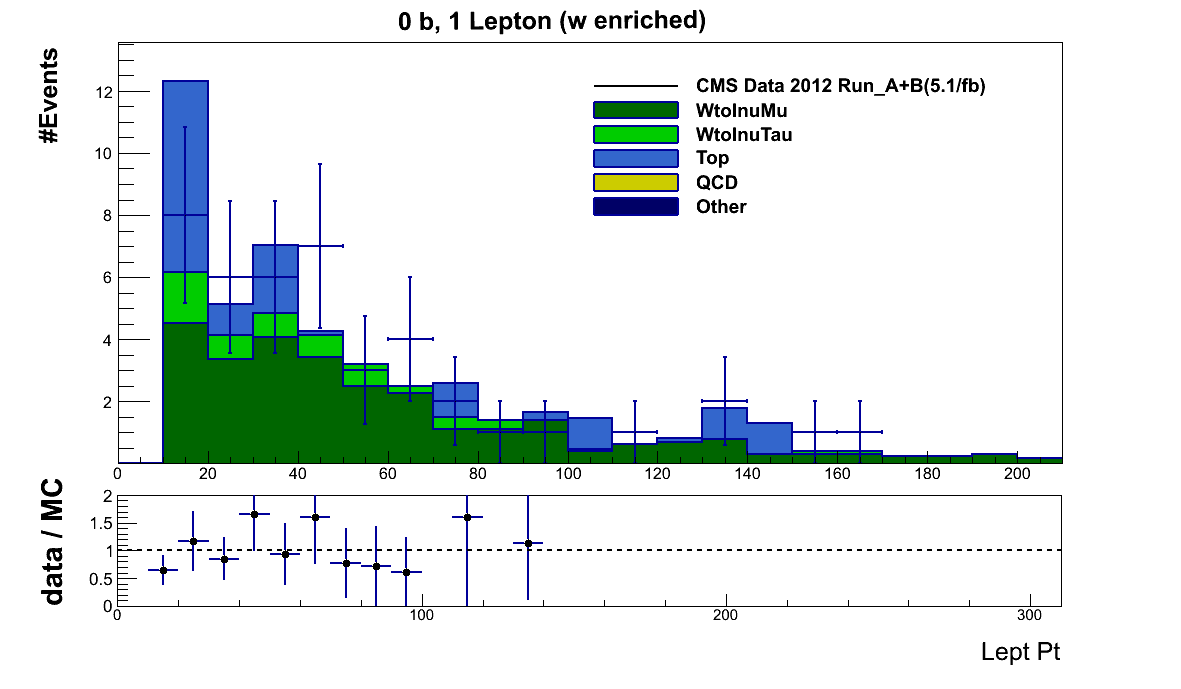
\includegraphics[angle=00,width=0.5\textwidth]{figs/Lept_Pt_0b_Mod.png}&
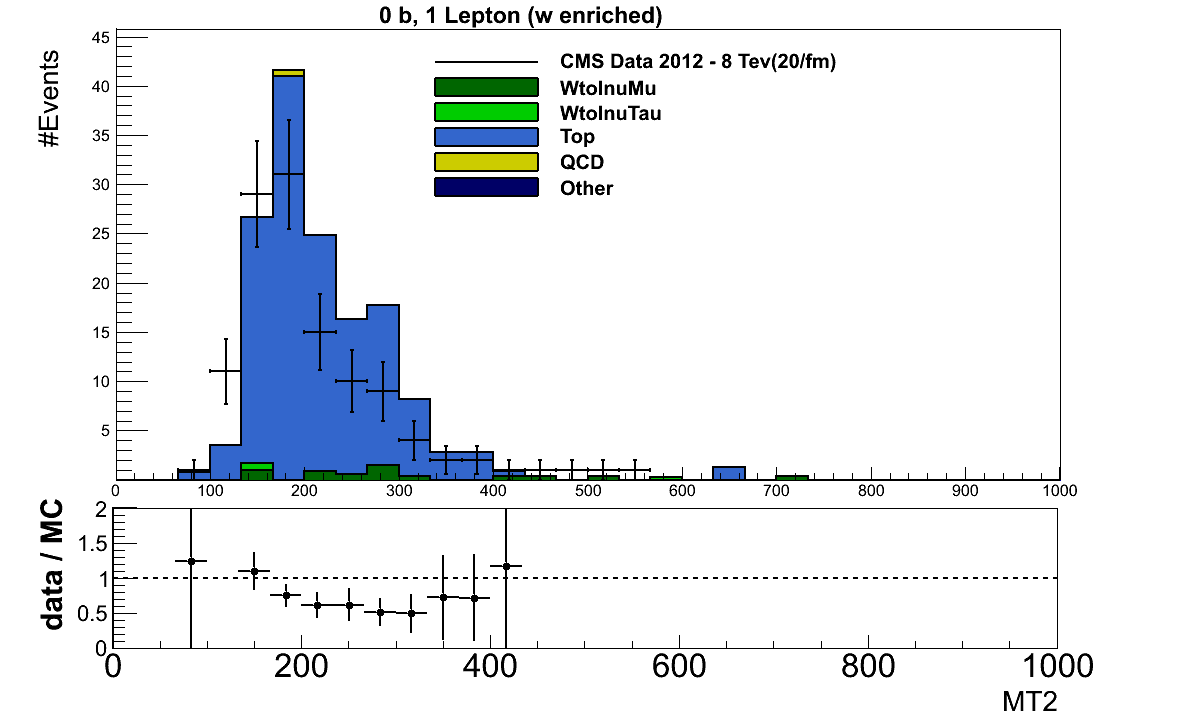
\includegraphics[angle=00,width=0.5\textwidth]{figs/MT2_0b_Mod.png}\\
	\mbox{\small{(a)}} & \mbox{\small{(b)}} \\
\end{array}$
\end{center}
\begin{center}$
\begin{array}{c}
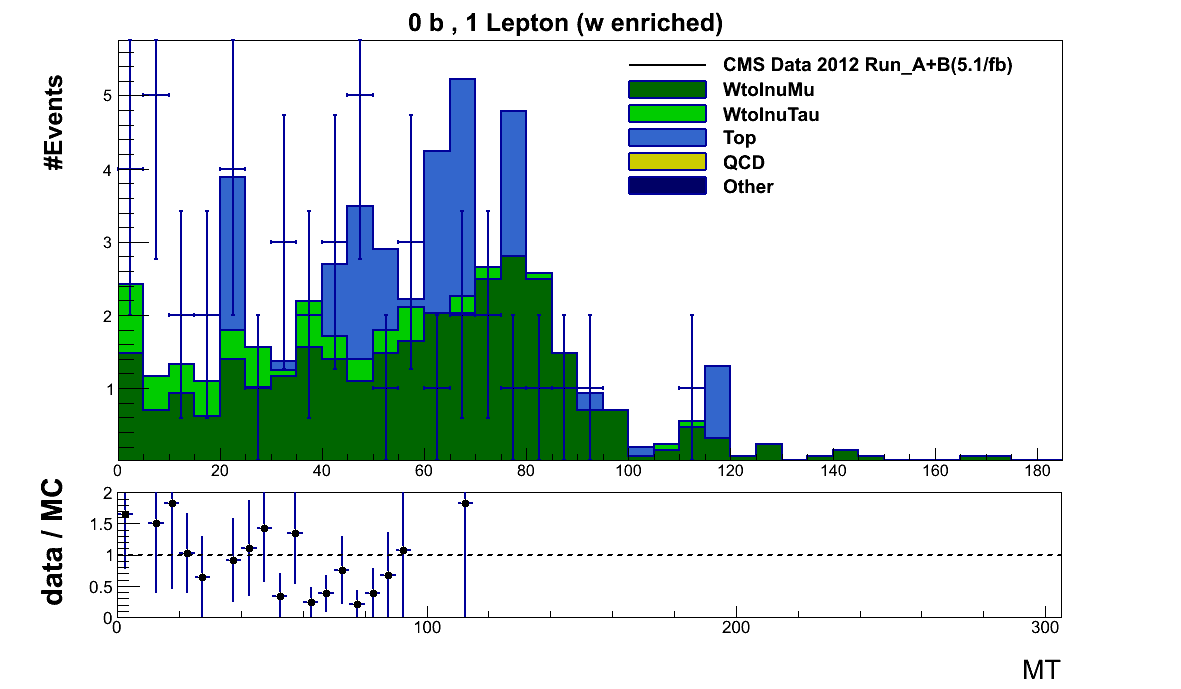
\includegraphics[angle=00,width=0.5\textwidth]{figs/MT_0b_Mod.png}\\
	\mbox{\small{(c)}}  \\
\end{array}$
\end{center}
\caption{Muon \pT, \mttwo and \mt distributions for W-enriched region}
\label{fig:WenrichedPlots}

\end{figure}


%..........................
\begin{table}[!htb]
\setlength{\tabcolsep}{2pt}
\small
\begin{center}

\begin{tabular}{lccccccccc} 
\hline\hline
& WtolnuMu& WtolnuTau& QCD& Zinv& Top& SMS& Other& MC& data \\ \hline \hline
 All events ($\rm jets\geq X$) & 48.82  & 100.82  & 694.69  & 76.77  & 433.77  & 0.07  & 60.14  & 1415.00 $\pm$ 96.77 & 1172.00  \\ 
% $Minimum DPhi(\met,jet) > 0.3$ & 40.56  & 65.36  & 146.80  & 65.29  & 328.56  & 0.06  & 50.78  & 697.35 $\pm$ 52.10 & 597.00  \\ 
 %HBHE noise veto & 40.56  & 65.36  & 146.80  & 65.29  & 328.56  & 0.06  & 50.78  & 697.35 $\pm$ 52.10 & 597.00  \\ 
 %$\met > 30GeV$ & 40.56  & 65.36  & 146.80  & 65.29  & 328.56  & 0.06  & 50.78  & 697.35 $\pm$ 52.10 & 597.00  \\ 
 %$VectorSumPt < 70$ & 40.56  & 65.36  & 146.80  & 65.29  & 328.56  & 0.06  & 50.78  & 697.35 $\pm$ 52.10 & 597.00  \\ 
 Analysis selection cuts & 40.56  & 65.36  & 146.80  & 65.29  & 328.56  & 0.06  & 50.78  & 697.35 $\pm$ 52.10 & 597.00  \\ 
 Lepton Veto & 40.56  & 60.29  & 146.80  & 65.18  & 257.98  & 0.06  & 26.09  & 596.90 $\pm$ 51.43 & 531.00  \\ 
 Lepton Selection & 24.57  & 4.91  & 0.00  & 0.00  & 58.20  & 0.00  & 0.00  & 87.69 $\pm$ 7.51 & 66.00  \\ 
 $m_T < 100\rm \,GeV$ & 23.56  & 4.76  & 0.00  & 0.00  & 52.69  & 0.00  & 0.00  & 81.01 $\pm$ 7.16 & 58.00  \\ 
 $b$-jet Veto & 18.64  & 3.67  & 0.00  & 0.00  & 7.83  & 0.00  & 0.00  & 30.15 $\pm$ 2.95 & 29.00  \\ 
 \mttwo  100 - 150 GeV & 2.26  & 0.08  & 0.00  & 0.00  & 0.99  & 0.00  & 0.00  & 3.33 $\pm$ 1.08 & 1.00  \\ 
 \mttwo  150 - 200 GeV & 5.54  & 1.09  & 0.00  & 0.00  & 1.97  & 0.00  & 0.00  & 8.60 $\pm$ 1.57 & 10.00  \\ 
 \mttwo  200 - 275 GeV & 4.76  & 1.17  & 0.00  & 0.00  & 2.90  & 0.00  & 0.00  & 8.83 $\pm$ 1.60 & 7.00  \\ 
 \mttwo  275 - 375 GeV & 2.57  & 0.78  & 0.00  & 0.00  & 1.97  & 0.00  & 0.00  & 5.33 $\pm$ 1.49 & 5.00  \\ 
 \mttwo  375 - 500 GeV & 2.11  & 0.39  & 0.00  & 0.00  & 0.00  & 0.00  & 0.00  & 2.50 $\pm$ 0.44 & 4.00  \\ 
 $M_{T2} > 500$ GeV & 1.25  & 0.16  & 0.00  & 0.00  & 0.00  & 0.00  & 0.00  & 1.40 $\pm$ 0.33 & 1.00  \\ 
\hline\hline 
\end{tabular} 
\caption{Yields for the W-enriched selection}
\label{tab:WenrichYields}
\end{center} 
\end{table}

\subsubsection{\texorpdfstring{$\rm{t\bar{t}}$ background estimation in W-enriched sample}{tt background estimation in W-enriched sample}}

Despite of b-tag veto some top events remain in W enriched region. The contribution of $t\bar{t}$ is estimated from data while for the rest of backgrounds we trust on simulation. The b-tag veto is relaxed and at least one b-jet is requested to obtain a sample enriched in top events. The selection results are shown in Table~\ref{tab:toEnrichyields}. To find out the number top events in b-tag veto region (W enriched), b-tagging (in)efficiency has to be considered. This process can be described as:
%.................
\begin{linenomath}
\begin{equation}
\label{eq:topEst}
N_{top}(b-veto) = N_{top}(\geq1b-tag) \frac{\epsilon(b-veto)}{\epsilon(\geq1b-tag)},
\end{equation}
\end{linenomath}
where the $\epsilon(b-veto)$ and $\epsilon(\geq1b-tag)$ are the efficiencies of vetoing or selecting b-tagged events and are taken from simulation, thus corrected by the data-simulation scale factors given by the b-tag POG for the CSVE (0.963 $\pm$ 0.020) and CSVT(0.947 $\pm$ 0.025) working points, respectively~\cite{CMS-BTV-AN-12-470}. As it is apparent form Table~\ref{tab:toEnrichyields} there is a good agreement between data and MC in top-enriched region and also the Muon \pT, \mttwo and \mt distributions are shown in Figures~\ref{fig:topEnrichedPlots}a,~\ref{fig:topEnrichedPlots}b and~\ref{fig:topEnrichedPlots}c, respectively.


\begin{figure}[!h]
\begin{center}$
\begin{array}{cc} 
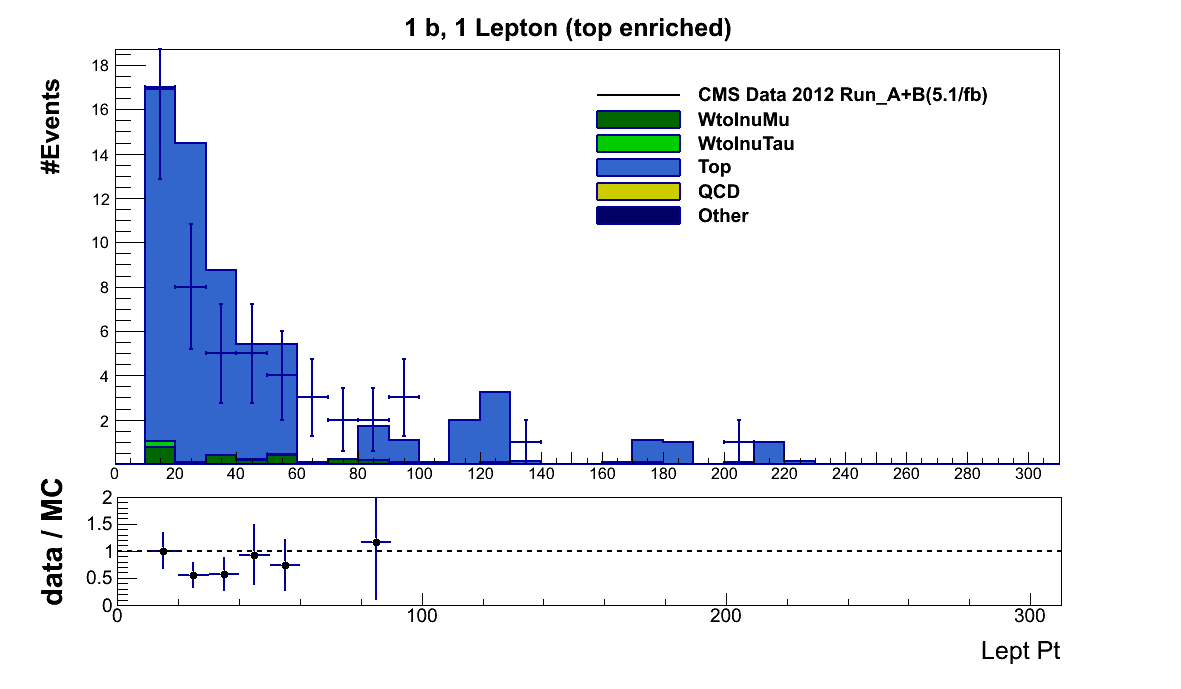
\includegraphics[angle=00,width=0.5\textwidth]{figs/Lept_Pt_1b_Mod.png}&
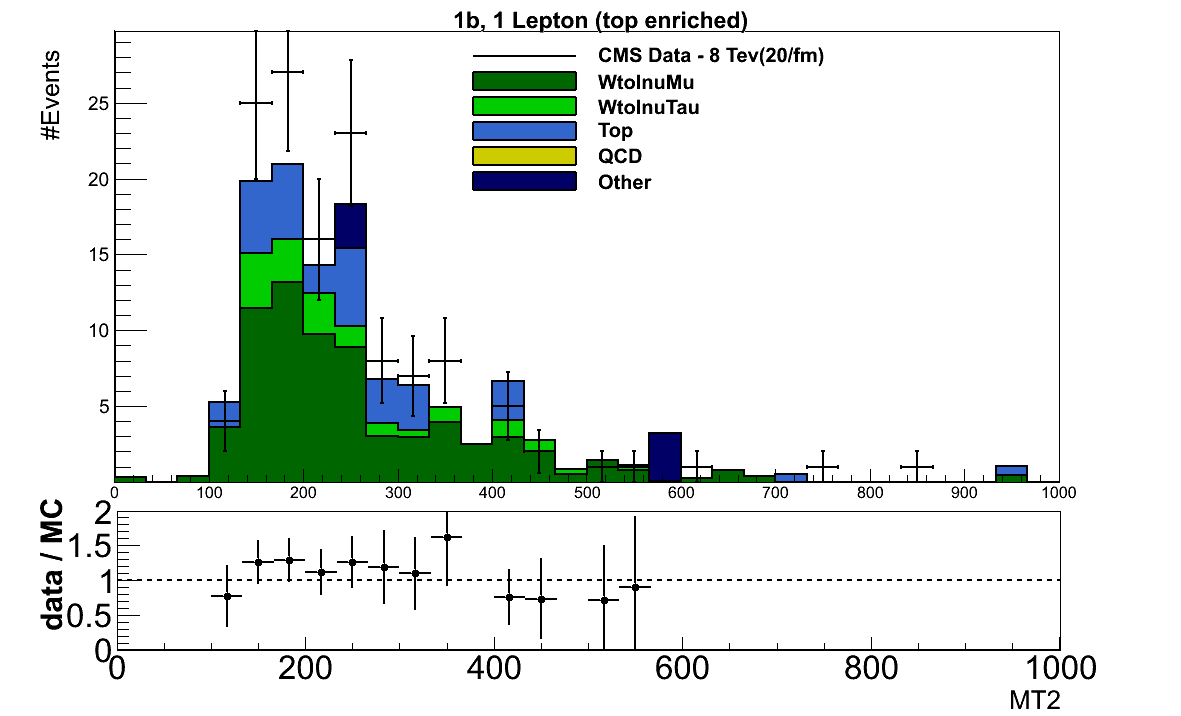
\includegraphics[angle=00,width=0.5\textwidth]{figs/MT2_1b_Mod.png}\\
	\mbox{\small{(a)}} & \mbox{\small{(b)}} \\
\end{array}$
\end{center}
\begin{center}$
\begin{array}{c}
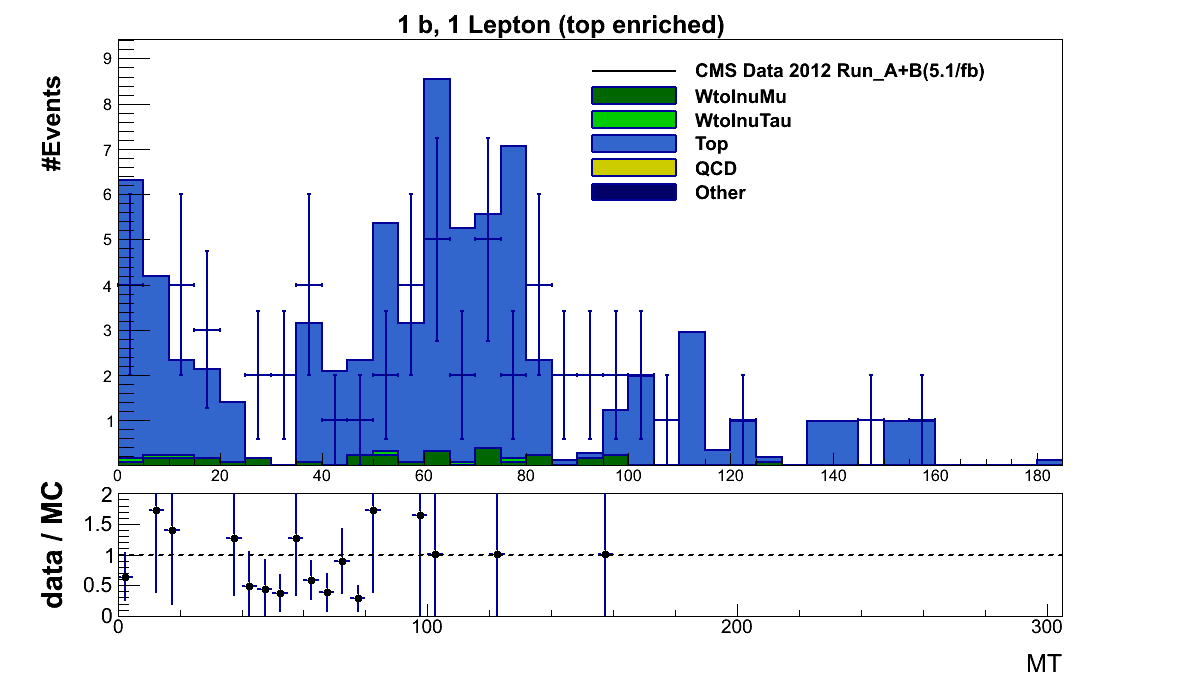
\includegraphics[angle=00,width=0.5\textwidth]{figs/MT_1b_Mod.png}\\
	\mbox{\small{(c)}}  \\
\end{array}$
\end{center}
\caption{Muon \pT, \mttwo and \mt distributions for top-enriched region}
\label{fig:topEnrichedPlots}
\end{figure}

%.....................
\begin{table}[!htb]
\setlength{\tabcolsep}{2pt}
\small
\begin{center} 

\begin{tabular}{lccccccccc} 
\hline\hline
& WtolnuMu& WtolnuTau& QCD& Zinv& Top& SMS& Other& MC& data \\ \hline \hline
 All events ($\rm jets\geq X$) & 48.82  & 100.82  & 694.69  & 76.77  & 433.77  & 0.07  & 60.14  & 1415.00 $\pm$ 96.77 & 1172.00  \\ 
 %$Minimum DPhi(\met,jet) > 0.3$ & 40.56  & 65.36  & 146.80  & 65.29  & 328.56  & 0.06  & 50.78  & 697.35 $\pm$ 52.10 & 597.00  \\ 
 %HBHE noise veto & 40.56  & 65.36  & 146.80  & 65.29  & 328.56  & 0.06  & 50.78  & 697.35 $\pm$ 52.10 & 597.00  \\ 
 %$\met > 30GeV$ & 40.56  & 65.36  & 146.80  & 65.29  & 328.56  & 0.06  & 50.78  & 697.35 $\pm$ 52.10 & 597.00  \\ 
% $VectorSumPt < 70$ & 40.56  & 65.36  & 146.80  & 65.29  & 328.56  & 0.06  & 50.78  & 697.35 $\pm$ 52.10 & 597.00  \\ 
Analysis selection cuts & 40.56  & 65.36  & 146.80  & 65.29  & 328.56  & 0.06  & 50.78  & 697.35 $\pm$ 52.10 & 597.00  \\ 
 Lepton Veto & 40.56  & 60.29  & 146.80  & 65.18  & 257.98  & 0.06  & 26.09  & 596.90 $\pm$ 51.43 & 531.00  \\ 
 Lepton Selection & 24.57  & 4.91  & 0.00  & 0.00  & 58.20  & 0.00  & 0.00  & 87.69 $\pm$ 7.51 & 66.00  \\ 
 $m_T < 100\, \rm GeV$ & 23.56  & 4.76  & 0.00  & 0.00  & 52.69  & 0.00  & 0.00  & 81.01 $\pm$ 7.16 & 58.00  \\ 
 $b$-jets Selection & 2.03  & 0.39  & 0.00  & 0.00  & 36.91  & 0.00  & 0.00  & 39.33 $\pm$ 5.95 & 21.00  \\ 
 \mttwo  100 - 150 GeV & 0.23  & 0.08  & 0.00  & 0.00  & 8.01  & 0.00  & 0.00  & 8.32 $\pm$ 2.80 & 7.00  \\ 
 \mttwo  150 - 200 GeV & 0.47  & 0.16  & 0.00  & 0.00  & 10.97  & 0.00  & 0.00  & 11.59 $\pm$ 3.28 & 5.00  \\ 
 \mttwo  200 - 275 GeV & 0.47  & 0.08  & 0.00  & 0.00  & 11.78  & 0.00  & 0.00  & 12.32 $\pm$ 3.30 & 9.00  \\ 
 \mttwo  275 - 375 GeV & 0.47  & 0.00  & 0.00  & 0.00  & 3.08  & 0.00  & 0.00  & 3.54 $\pm$ 1.72 & 0.00  \\ 
 \mttwo  375 - 500 GeV & 0.16  & 0.00  & 0.00  & 0.00  & 2.96  & 0.00  & 0.00  & 3.12 $\pm$ 1.71 & 0.00  \\ 
 $M_{T2} > 500$ GeV & 0.23  & 0.08  & 0.00  & 0.00  & 0.12  & 0.00  & 0.00  & 0.43 $\pm$ 0.19 & 0.00  \\ 
\hline\hline 
\end{tabular} 
\caption{Yields for the top-enriched selection}
\label{tab:toEnrichyields}
\end{center} 
\end{table}


%...........................
\subsubsection{Z Estimation Results}
After finding the number of top events in the b-tag veto (W-enriched) region, it is subtracted from the number of W's of this region, derived from data, to obtain the correct number of $W\rightarrow\mu\nu$ events. Due to requesting one b-jet in the final state we need to have the number of W's in 1 b-tag region to be able to estimate the number of Z in this region. Therefore we must multiply the number of W's in b-tag veto region to $\frac{\epsilon(1b W)}{\epsilon(0b W)}$ to reach the number of W's in 1 b-tag region and this ratio is coming from MC and it is considered b-tag scale factor.   

\subsubsection{Systematic uncertainties}
\label{subsect:ZnnSyst}
The systematic uncertainty on $Z\to \nu\nu$ estimation has contributions from different sources, as can be seen in Equation~\ref{eq:ZinvEst}. There, the uncertainty on $R^{MC}$ is taken from simulation where it includes the uncertainties due to the PDF set and the k-factor [FIXME?] in Z and W bosons production rates. The uncertaintiy on the muon acceptance efficiency is derived from simulation, too. The muon selection efficiency ($\epsilon_{reco/iso}$) as well as its uncertainty are data-driven, obtained from the Tag\&Probe method. Another uncertainty in this estimation arises from the requirement of $m_T<100\,\rm GeV$ which is estimated from simulation.\\
For the $N_{W(\mu\nu)}$ in the analysis region with at least one b-tagged jet, the $N_{W(\mu\nu)}$ estimation in b-tag veto region is corrected with  the data-driven b-tagging and b-tag veto efficiencies. The uncertainties on these efficiencies are taken from data, accordingly.\\
Other than $t\bar{t}$, all backgrounds and their uncertainties are estimated from simulation in $N_{W(\mu\nu)}$ calculation. The $t\bar{t}$ contribution in W-enriched (b-tag veto) region is obtained using Equation~\ref{eq:topEst}. In this estimation, the uncertainties on b-tagging efficiencies are taken from data while the background uncertanties are derived from simulation. \\ 

The final estimation together with their uncertainties are summarized in Table~\ref{tab:ZinvFinalRes}.

\begin{table}[!htb]
\small
\setlength{\tabcolsep}{20pt} 
\begin{center} 
\begin{tabular}{lccccccc} 
\hline\hline
&                 &    MC                     & Data Estimation\\\hline \hline
& top  (0b, 1l)     & 7.83 $\pm$ 2.64             &4.17 $\pm$ 2.09 ( 0.91 (stat) $\pm$ 1.88 (syst))\\
&  W   (0b, 1l)     & 18.64 $\pm$ 1.21            & 21.35 $\pm$ 5.05 ( 4.07 (stat) $\pm$ 2.99 (syst))\\ 
& Zinv (1b, 0l)           &  5.62 $\pm$ 0.39            &6.99 $\pm$ 2.50 ( 1.33 (stat) $\pm$ 2.11 (syst))\\
\hline\hline 
\end{tabular} 
\caption{Z-invisible Estimation}
\label{tab:ZinvFinalRes}
\end{center} 
\end{table}
